\section{Positive flux and finite strip transfers}\label{sec:flux}

We write
\begin{equation}\label{eq:01-constants}
 t=\frac38,\qquad \lambda=\frac\pi8,\qquad
 d=\cos(2\lambda)=\sin(2\lambda),\qquad C=\cos\lambda.
\end{equation}
Then $c=\cos(3\lambda)$ and $\rho=C-c=1/(2C)$, consistently
with \eqref{eq:critical-weight}.

The boundary identity controls positive path sums before any spectral parameter is introduced. We use it first to make the fixed-height transfer construction convergent. The local identities then allow the stationary vector to be recovered by polynomial interpolation.


\begin{lemma}[Boundary identity]\label{lem:boundary-flux}
Let $D$ be a finite simply connected union of triangles with simple
polygonal boundary, and let $a$ be a boundary port. If $W(\gamma)$ is
the total signed turning of a path, measured from its inward initial
direction to its outward final direction, then
\begin{equation}\label{eq:01-boundary-identity}
 \sum_{b\in\partial D}\ \sum_{\gamma:a\to b}
       \rho^{|\gamma|}e^{itW(\gamma)}=1.
\end{equation}
If $D$ is convex, its unsigned boundary partition sum is at most $1/c$.
\end{lemma}

\begin{proof}
Send mass one along the inward half-edge at $a$. At each newly visited
vertex split it between the two possible continuations, multiplying by
$\rho e^{i\lambda}$ and $\rho e^{-i\lambda}$, respectively. The identity
$2\rho\cos\lambda=1$ conserves total mass. Stop a branch when it exits
$D$ or is about to enter a vertex already visited. This produces a finite
tree because $D$ has finitely many vertices.

For a stopped collision, the newly closed cycle is simple and has a
disjoint incoming stem. The stem lies outside the cycle: it starts on
$\partial D$ and cannot cross the cycle before their first common
vertex. Consequently the unused branch at that vertex is exterior to
the cycle. The cycle turn there is $\pi/3$ in the counterclockwise
orientation, rather than $-\pi/3$; the clockwise statement is reversed.
The turn from the stem into the cycle replaces this closing turn by its
negative. The two ways to traverse the cycle therefore have winding
increments $4\pi/3$ and $-4\pi/3$ relative to the stem. They have the
same unsigned weight and cancel, since
$e^{it(4\pi/3)}+e^{-it(4\pi/3)}=0$. Cycle reversal is an involution on
all stopped collisions. The remaining terminal mass gives
\eqref{eq:01-boundary-identity}.

For a path ending at $b$, close it using the counterclockwise boundary
arc from $b$ to $a$. The turns at the two ports are $\pi/2$, so the
turning theorem for this simple closed curve gives
\[
 W(\gamma)=\pi-\operatorname{turn}_{\partial D}(b\to a).
\]
For a convex boundary the latter turn lies in $[0,2\pi]$. Thus
$|W(\gamma)|\le\pi$ and
$\cos(tW(\gamma))\ge\cos(3\pi/8)=c$.
Taking real parts proves the last assertion.
\end{proof}

We next introduce auxiliary spectral parameters. A column has $N$
rhombi stacked along horizontal edges; in row $i$ the other edge makes
angle $u_i/t$ with the horizontal. The same tiles make sense as
combinatorial diagrams for complex $u_i$. Their four ports carry
noncrossing partial pairings. Port occupancies must agree when tiles
are glued, and every closed component has weight zero. Put
\begin{equation}\label{eq:01-rhombic-weights}
\begin{aligned}
 a(u)&=\cos(2u-3\lambda),&
 L(u)&=\sin(2\lambda+u)\sin(3\lambda+u)=\frac{C+a(u)}2,\\
 A(u)&=\frac{d\sin(3\lambda-u)}{L(u)},&
 U(u)&=\frac{d\sin u}{L(u)},\\
 B(u)&=\frac{\sin u\sin(3\lambda-u)}{L(u)}
       =\frac{a(u)-c}{a(u)+C},\\
 E(u)&=\frac{\sin(3\lambda-u)\sin(2\lambda-u)}{L(u)},&
 F(u)&=\frac{\sin(u-\lambda)\sin u}{L(u)}.
\end{aligned}
\end{equation}
These weights come from Nienhuis's integrable $O(n)$ construction
\cite{Nienhuis1990CriticalMulticritical}, in the self-avoiding-walk
normalization displayed in \cite{GM2019}; the general parafermionic and integrable local formulas
are discussed in \cite{IkhlefCardy2009,Glazman2015}.
The empty tile has weight one. A single connection between opposite
ports has weight $B$. A bottom--left or top--right turn has weight $A$;
the other two turns have weight $U$. The configurations with two turns
of the first or second type have weights $E$ and $F$, respectively.
At $u=\lambda$ or $2\lambda$, splitting along the short diagonal recovers
two triangular tiles, with weight $\rho$ per visited triangle. At
$u=0$ or $3\lambda$ the row is flat: each route continues deterministically
through the adjacent left or right port, and the two disjoint routes
can coexist with weight one.

The dilute diagram algebra and its Yang--Baxter operators have an
algebraic construction in Grimm and Pearce~\cite{GrimmPearce1993}.
Their distinction between gauge-invariant periodic partition functions
and other gauge-dependent quantities is relevant here: we specify the caps, scalar factors
and port ordering, and prove the identities for these choices.

We use the planar diagram algebra whose inputs and outputs are ordered
slots, each vacant or occupied. Composition glues matching slots and
annihilates a mismatch or a closed loop. Tensor product means
juxtaposition; transpose reflects a diagram, interchanging inputs and
outputs. The two-slot operator $R(v)$ has coefficients
$1,A(v),B(v),U(v),E(v),F(v)$ on, respectively, the empty diagram, a
single vertical connection, a single diagonal connection, a cap alone
or cup alone, two vertical connections, and a cap together with a cup.
There are two choices for a single vertical or diagonal connection, as
shown in Figure~\ref{fig:local-operator}.

\begin{figure}[htbp]
\centering
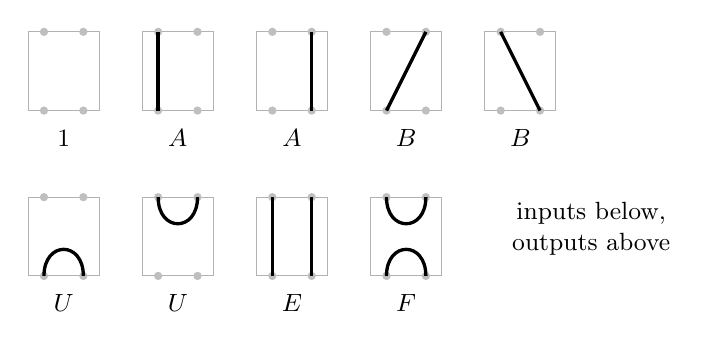
\begin{tikzpicture}[x=1cm,y=1cm,font=\small]
\foreach \j/\wt in {0/1,1/A,2/A,3/B,4/B,5/U,6/U,7/E,8/F}{
 \begin{scope}[xshift={1.45*mod(\j,5)*1cm},yshift={-2.1*floor(\j/5)*1cm}]
 \draw[black!30] (-.45,0) rectangle (.45,1);
 \foreach \x in {-.25,.25}{\fill[black!25] (\x,0) circle (1.5pt);\fill[black!25] (\x,1) circle (1.5pt);}
 \ifnum\j=1 \draw[very thick] (-.25,0)--(-.25,1);\fi
 \ifnum\j=2 \draw[very thick] (.25,0)--(.25,1);\fi
 \ifnum\j=3 \draw[very thick] (-.25,0)--(.25,1);\fi
 \ifnum\j=4 \draw[very thick] (.25,0)--(-.25,1);\fi
 \ifnum\j=5 \draw[very thick] (-.25,0) .. controls (-.25,.45) and (.25,.45) .. (.25,0);\fi
 \ifnum\j=6 \draw[very thick] (-.25,1) .. controls (-.25,.55) and (.25,.55) .. (.25,1);\fi
 \ifnum\j=7 \draw[very thick] (-.25,0)--(-.25,1) (.25,0)--(.25,1);\fi
 \ifnum\j=8 \draw[very thick] (-.25,0) .. controls (-.25,.45) and (.25,.45) .. (.25,0);\draw[very thick] (-.25,1) .. controls (-.25,.55) and (.25,.55) .. (.25,1);\fi
 \node at (0,-.35) {$\wt$};
 \end{scope}
}
\node[align=center] at (6.7,-1.5) {inputs below,\\outputs above};
\end{tikzpicture}
\caption{The nine local diagrams of $R(v)$, with coefficients evaluated
at $v$. Grey dots mark available slots; a slot is occupied exactly when a
black strand meets it. Gluing requires matching occupancies and assigns
zero to every closed component. These are operator diagrams, rather than
a geometric drawing of a rhombus.}
\label{fig:local-operator}
\end{figure}


Number the rows from bottom to top. A column swept from left to right
uses $R(3\lambda-u_i)$ in row $i$, with local ordered inputs
(south, west) and outputs (east, north). The north output of row $i$
is the south input of row $i+1$. The geometric and operator weights agree
because
\[
 A(3\lambda-u)=U(u),\quad U(3\lambda-u)=A(u),\quad
 B(3\lambda-u)=B(u),\quad E(3\lambda-u)=F(u).
\]
The last relation also gives $F(3\lambda-u)=E(u)$.
Figure~\ref{fig:rhombus-dictionary} records the port order.

\begin{figure}[htbp]
\centering
\begin{tikzpicture}[x=1.2cm,y=1.2cm,font=\small,>=Latex]
 \draw[thick] (0,0)--(1.2,0)--(1.8,1.039)--(.6,1.039)--cycle;
 \foreach \x/\y/\label/\pos in {.6/0/south/below,.3/.5195/west/left,1.5/.5195/east/right,1.2/1.039/north/above}{
  \draw[fill=white] (\x,\y) circle (2pt);
  \node[\pos=3pt] at (\x,\y) {\label};
 }
 \draw[->] (.38,0) arc[start angle=0,end angle=60,radius=.38];
 \node at (.66,.23) {$u/t$};
 \draw[->] (2.25,.52)--(3.1,.52);
 \draw[black!50] (3.55,0) rectangle (4.75,1.039);
 \node at (4.15,.52) {$R(3\lambda-u)$};
 \foreach \x/\y/\label/\pos in {3.75/0/south/below,4.55/0/west/below,3.75/1.039/east/above,4.55/1.039/north/above}{
  \fill (\x,\y) circle (1.5pt);
  \node[\pos=3pt] at (\x,\y) {\label};
 }
\end{tikzpicture}
\caption{From a geometric rhombus to a column operator. South and west
are the ordered inputs; east and north are the ordered outputs. The
operator is drawn with its inputs below and outputs above, so the
rhombic parameter $u$ corresponds to the operator argument $3\lambda-u$.
The rhombus is schematic; only the angle label and port order matter.}
\label{fig:rhombus-dictionary}
\end{figure}



Define $S_2$, from one slot to two, by sending a vacancy to a vacancy
plus $\rho$ times a cup, and an occupied strand to either output slot
with coefficient $\rho$. Define $S_3$, from no slots to two, to be the
sum of the vacant diagram and a cup.

\begin{lemma}[Local diagram identities]\label{lem:local-identities}
Writing $R_i$ for action in slots $i,i+1$, one has
\begin{align}
 R_2(y)R_1(x+y)R_2(x)&=R_1(x)R_2(x+y)R_1(y),
       \label{eq:01-braid}\\
 R(s\lambda)&=S_sS_s^{\mathsf t},\qquad s=2,3,
       \label{eq:01-factorization}\\
 R_2(x)R_1(x+s\lambda)(I\otimes S_s)
       &=(S_s\otimes I)\widehat R_s(x),
       \label{eq:01-splitting}\\
 R(x)R(-x)&=I.\label{eq:01-unitarity}
\end{align}
Here $\widehat R_2(x)=R(x+\lambda)$ and $\widehat R_3(x)$ is the
one-slot identity. These are identities of rational functions. They
can be specialized wherever the relevant sides are regular, including
at removable singularities; an individual operator at a genuine pole
is not assigned a finite value.
\end{lemma}

The complete coefficient proof is in Appendix~\ref{app:local-calculations}.


For a cut between two columns of $N$ rows, number its slots from
bottom to top. Let $\mathcal L_N^0$ be the vector space with basis the
noncrossing partial pairings of occupied slots; all other slots are
vacant. Let $\mathcal L_N^1$ have the same pairings with one additional
unpaired occupied slot connected to an exterior source. This defect
cannot be enclosed by a pair. Restricting a single path to one side
of a cut can produce several paired fragments as well as the
source-connected strand, as Figure~\ref{fig:cut-states} illustrates.

\begin{figure}[htbp]
\centering
\begin{tikzpicture}[x=1.45cm,y=1.45cm,font=\small,>=Latex]
 \draw[black!55] (-2.1,0)--(2.65,0);
 \draw[dashed,black!50] (0,-.12)--(0,3.05);
 \node[above] at (0,3.05) {cut};
 \node at (-1.3,2.95) {left source state};
 \node at (1.65,2.95) {right source state};
 \draw[very thick,blue!65!black]
   (-1.65,0) .. controls (-1.65,.38) and (-.45,.45) .. (0,.45)
   .. controls (.58,.45) and (.58,.9) .. (0,.9)
   .. controls (-.58,.9) and (-.58,1.35) .. (0,1.35)
   .. controls (1.05,1.35) and (1.05,2.25) .. (0,2.25)
   .. controls (-.58,2.25) and (-.58,2.7) .. (0,2.7)
   .. controls (1.3,2.7) and (2.3,2.7) .. (2.3,2.35)
   -- (2.3,0);
 \foreach \j/\y in {1/.45,2/.9,3/1.35,5/2.25,6/2.7}{
  \fill[blue!65!black] (0,\y) circle (2pt);
  \node[anchor=south east,inner sep=2pt] at (0,\y) {$\j$};
 }
 \draw[black!50,fill=white] (0,1.8) circle (2pt);
 \node[anchor=east] at (-.07,1.8) {$4$ vacant};
 \draw[thick,fill=white] (-1.65,0) circle (2pt);
 \draw[thick,fill=white] (2.3,0) circle (2pt);
 \node[below=3pt] at (-1.65,0) {$a$};
 \node[below=3pt] at (2.3,0) {$b$};
\end{tikzpicture}
\caption{A single arch may cross a cut several times. In this schematic
example the left half has a source strand at slot $1$ and pairs $(2,3)$,
$(5,6)$; the right half has pairs $(1,2)$, $(3,5)$ and a source strand
at slot $6$. Slot $4$ is vacant on both sides. Each source strand is
exposed, meaning that no pair encloses its slot. Gluing the two states
recovers one path from $a$ to $b$, with no closed component.}
\label{fig:cut-states}
\end{figure}


Before fixing its two auxiliary ends, the complete column is the map
\begin{equation}\label{eq:full-column}
 M_X=R_N(v_N)\cdots R_1(v_1),\qquad
 v_i=3\lambda-u_i,\qquad X=(u_1,\ldots,u_N).
\end{equation}
Its ordered inputs are $(\mathrm{aux},1,\ldots,N)$ and its ordered
outputs are $(1,\ldots,N,\mathrm{aux})$: the auxiliary slot moves from
the south end to the north end of the column. Attach a cut state to
the west inputs, glue matching occupancies, and record the east state,
assigning zero to any closed loop. With both auxiliary ends vacant,
this defines $T_N^{(\epsilon)}:\mathcal L_N^\epsilon\to
\mathcal L_N^\epsilon$, $\epsilon=0,1$; write $T_N=T_N^{(0)}$.
With the south end occupied and the north end vacant, it defines the
source insertion $\mathsf b_N:\mathcal L_N^0\to\mathcal L_N^1$.
Interchanging these end conditions defines $\mathsf b_N^{\rm north}$.
A superscript $-$ denotes the corresponding maps for a sweep from
right to left. Horizontal reflection replaces $X$ by
$X^*=(3\lambda-u_1,\ldots,3\lambda-u_N)$, so its complete column is
$M_X^-=R_N(u_N)\cdots R_1(u_1)$.
The empty coordinate of $T_Nv$ equals that of $v$: any occupied input
that closed up before reaching an output would form a forbidden loop.

\noindent\begin{minipage}{\linewidth}
\begin{lemma}[Decay and rational continuation]\label{lem:transfer-decay}
If every $u_i$ belongs to $\{0,\lambda,2\lambda,3\lambda\}$, then
$T_N$ restricted to vectors with zero empty coordinate and
$T_N^{(1)}$ have spectral radius strictly less than one. The same
holds for reversed columns and in a complex neighborhood of each
such parameter list, with absolute values of tile weights used to
control absolute convergence.

There is consequently a unique stationary vacuum vector $P_N$ with
empty coordinate one. Its entries are rational in the $e^{iu_i}$,
and regular at every parameter list just specified.
\end{lemma}
\end{minipage}\par

\begin{proof}
First take a homogeneous triangular parallelogram of height $H>0$
and width $M$. The total weight of paths from a fixed left port to
its right side tends to zero as $M\to\infty$. To see this, append a
column immediately to the right of the exit and continue, entirely
inside this new column, to its bottom port. The continuation has at most a fixed number
of vertices depending only on $H$, so its weight is bounded below
by a positive constant depending only on $H$. For every $M<L$ these
extensions are paths in a parallelogram of width $L$. Their bottom
endpoints identify $M$, and their first exit into the appended
column recovers the original path. They are therefore distinct.
Writing $q_H(M)$ for the crossing mass and $C_H$ for the maximum
number of added vertices, Lemma~\ref{lem:boundary-flux} gives
\[
 \rho^{C_H}\sum_{M<L}q_H(M)\le 1/c.
\]
Thus $q_H(M)\to0$. The same lemma uniformly bounds paths joining
ports on the same side.

For a mixed list of the four allowed parameters, collapse the flat
rows. The row vectors belong to
$\{1,e^{i\pi/3},e^{2i\pi/3},-1\}$, so outside two end pieces of
horizontal size $O(N)$ the remaining triangles form a homogeneous
parallelogram of height $H$, the number of nonflat rows, and width
$M-O(N)$. This description does not depend on which neighboring
triangles were grouped into rhombi. A collapsed deterministic route
drifts by at most $N$ columns. The end pieces have bounded size for
fixed $N$ and contribute bounded weights.

Every nonzero diagram contributing to either restricted transfer
power has a component connecting the left and right cuts. In the
vacuum sector, otherwise the nonempty input pairing would close
into a loop; in the source sector, the source must reach the output.
Cut all components at the two ends of the homogeneous core. There
are only boundedly many endpoint patterns, depending on $N$, and at
least one segment spans the core. Ignoring avoidance between these
segments bounds their total weight by a product of single-path
partition sums. Each nonspanning factor is at most $1/c$.
For $H>0$, choose the core width $M-\kappa_X$, where the fixed
offset satisfies $0\le\kappa_X=O(N)$. If $Q_N$ is the nonempty vacuum block and
$\|\cdot\|_{\max}$ is the maximum absolute matrix entry, then
\[
 \|Q_N^M\|_{\max}+\|(T_N^{(1)})^M\|_{\max}
 \le C_N\sum_{a\in\mathcal E_H}q_{H,a}(M-\kappa_X)\longrightarrow0.
\]
Here $\mathcal E_H$ is the finite set of left ports of the core,
$q_{H,a}$ is its crossing mass from $a$, and $C_N$ absorbs the bounded
end pieces and endpoint patterns. All constants are for fixed $N$;
no uniform spectral gap is needed. If $H=0$,
no spanning component is possible once $M$ is sufficiently large.
Thus both restricted matrix powers tend to zero. Since these are
finite matrices, their spectral radii are less than one.

At the specified parameters all tile weights are nonnegative. The
matrices obtained by taking absolute tile weights vary continuously,
so their restricted spectral radii remain less than one in a small
complex neighborhood. This also proves the asserted absolute
convergence. The reflected argument is identical.

Writing the vacuum matrix in the empty/nonempty decomposition gives
$T_N=\left(\begin{smallmatrix}1&0\\v&Q\end{smallmatrix}\right)$.
Its normalized stationary vector is $(1,(I-Q)^{-1}v)$, which is regular
in the stated neighborhoods and rational in the spectral variables.
This proves both uniqueness and the continuation claim. Equivalently,
$P_N$ is the sum of finite path diagrams in the vacuum half-strip.
\end{proof}

We now pass from local identities to column identities. This also
records the source insertions needed for the arch moment. Let $X'$ be
$X$ with adjacent rows $i,i+1$ exchanged, and put
$\delta=u_{i+1}-u_i$. Applying the braid relation to those rows gives
\begin{equation}\label{eq:column-exchange}
 M_X(I_{\rm aux}\otimes R_i(\delta))
 =(R_i(\delta)\otimes I_{\rm aux})M_{X'}.
\end{equation}
The tensor positions reflect the different input and output orders
in \eqref{eq:full-column}.
If $u_{i+1}=u_i+s\lambda$, $s=2,3$, let $X_{\rm red}$ replace these
rows by $u_i+\lambda$ for $s=2$, or delete them for $s=3$.
The splitter $S_s$ acts on these cut slots, with identities on all
other slots. In each sector it maps
$\mathcal L_{N-r_s}^\epsilon$ to $\mathcal L_N^\epsilon$, where
$r_2=1$ and $r_3=2$. The local splitting identity yields
\begin{equation}\label{eq:column-splitting}
 M_X(I_{\rm aux}\otimes S_s)
 =(S_s\otimes I_{\rm aux})M_{X_{\rm red}}.
\end{equation}
Indeed its argument is $x=v_{i+1}$, and for $s=2$ the effective box
has argument $x+\lambda=3\lambda-(u_i+\lambda)$, as required.
Transpose splitting and reverse the slot order to obtain the reflected
projection identity
\begin{equation}\label{eq:column-reflection}
 (S_s^{\mathsf t}\otimes I_{\rm aux})M_X^-
 =M_{X_{\rm red}}^-(I_{\rm aux}\otimes S_s^{\mathsf t}).
\end{equation}
All three equations leave the auxiliary endpoints untouched. We can
therefore impose either vacant ends or either source-insertion
condition. With $X$ as a subscript denoting its row list, this gives,
for $\epsilon=0,1$,
\begin{equation}\label{eq:transfer-intertwiners}
\begin{aligned}
 T_X^{(\epsilon)}R_i(\delta)&=R_i(\delta)T_{X'}^{(\epsilon)},&
 \mathsf b_XR_i(\delta)&=R_i(\delta)\mathsf b_{X'},\\
 T_X^{(\epsilon)}S_s&=S_sT_{X_{\rm red}}^{(\epsilon)},&
 \mathsf b_XS_s&=S_s\mathsf b_{X_{\rm red}},\\
 S_s^{\mathsf t}T_X^{(\epsilon),-}
 &=T_{X_{\rm red}}^{(\epsilon),-}S_s^{\mathsf t},&
 S_s^{\mathsf t}\mathsf b_X^-
 &=\mathsf b_{X_{\rm red}}^-S_s^{\mathsf t}.
\end{aligned}
\end{equation}
The same equations hold with $\mathsf b^{\rm north}$ in place of
$\mathsf b$. In a source-insertion equation the cut map on its right
acts in the vacuum sector and the cut map on its left acts in the
one-source sector.

The normalized stationary vector is now determined under exchange
and reduction:
\begin{align}
 P_N(\ldots,u_i,u_{i+1},\ldots)
 &=R_i(u_{i+1}-u_i)P_N(\ldots,u_{i+1},u_i,\ldots),
 \label{eq:01-vacuum-exchange}\\
 P_N&=S_sP_{\mathrm{red}}
 \quad\text{when }u_{i+1}=u_i+s\lambda.
 \label{eq:01-vacuum-reduction}
\end{align}
The column equations prove stationarity of the right sides. Their empty
coordinate is one: a cap producing an empty output from a nonempty
pairing would close a zero-weight loop. Uniqueness in
Lemma~\ref{lem:transfer-decay} proves exchange near the all-zero
parameter list, and reduction near a mixed list with $u_i=0$.
Intersecting these regular neighborhoods with the specialization
hypersurface gives an open set in that hypersurface. Rational
continuation then proves the identities for general parameters.
The reflected projection and source equations will be used in the
same way, with uniqueness of the corresponding stationary or
inhomogeneous transfer equation.

At $u_1=3\lambda$, the first slot is vacant and can be deleted. At
$u_1=0$, the part with first slot vacant is $P_{N-1}$; the occupied
part is obtained from $P_{N-1}$ by one column on rows $2,\ldots,N$
with a south source and vacant north, tying that source to slot $1$.
These assertions follow from $R(0)=I$ and
$R(3\lambda)=S_3S_3^{\mathsf t}$; in the latter identity an occupied
first input with vacant auxiliary input contributes zero.
Finally, shifting $u_k$ by $\pi$ multiplies each tile weight by the
occupancy signs at its west and east ports. Thus it conjugates $T_N$
by the diagonal map $D_k$ that changes the sign of states with slot
$k$ occupied. Since $D_k$ preserves the empty coordinate, uniqueness
gives $P_N(X+\pi e_k)=D_kP_N(X)$, where $e_k$ is the $k$th coordinate
vector.
